
% Default to the notebook output style

    


% Inherit from the specified cell style.




    
\documentclass[11pt]{article}

    
    
    \usepackage[T1]{fontenc}
    % Nicer default font (+ math font) than Computer Modern for most use cases
    \usepackage{mathpazo}

    % Basic figure setup, for now with no caption control since it's done
    % automatically by Pandoc (which extracts ![](path) syntax from Markdown).
    \usepackage{graphicx}
    % We will generate all images so they have a width \maxwidth. This means
    % that they will get their normal width if they fit onto the page, but
    % are scaled down if they would overflow the margins.
    \makeatletter
    \def\maxwidth{\ifdim\Gin@nat@width>\linewidth\linewidth
    \else\Gin@nat@width\fi}
    \makeatother
    \let\Oldincludegraphics\includegraphics
    % Set max figure width to be 80% of text width, for now hardcoded.
    \renewcommand{\includegraphics}[1]{\Oldincludegraphics[width=.8\maxwidth]{#1}}
    % Ensure that by default, figures have no caption (until we provide a
    % proper Figure object with a Caption API and a way to capture that
    % in the conversion process - todo).
    \usepackage{caption}
    \DeclareCaptionLabelFormat{nolabel}{}
    \captionsetup{labelformat=nolabel}

    \usepackage{adjustbox} % Used to constrain images to a maximum size 
    \usepackage{xcolor} % Allow colors to be defined
    \usepackage{enumerate} % Needed for markdown enumerations to work
    \usepackage{geometry} % Used to adjust the document margins
    \usepackage{amsmath} % Equations
    \usepackage{amssymb} % Equations
    \usepackage{textcomp} % defines textquotesingle
    % Hack from http://tex.stackexchange.com/a/47451/13684:
    \AtBeginDocument{%
        \def\PYZsq{\textquotesingle}% Upright quotes in Pygmentized code
    }
    \usepackage{upquote} % Upright quotes for verbatim code
    \usepackage{eurosym} % defines \euro
    \usepackage[mathletters]{ucs} % Extended unicode (utf-8) support
    \usepackage[utf8x]{inputenc} % Allow utf-8 characters in the tex document
    \usepackage{fancyvrb} % verbatim replacement that allows latex
    \usepackage{grffile} % extends the file name processing of package graphics 
                         % to support a larger range 
    % The hyperref package gives us a pdf with properly built
    % internal navigation ('pdf bookmarks' for the table of contents,
    % internal cross-reference links, web links for URLs, etc.)
    \usepackage{hyperref}
    \usepackage{longtable} % longtable support required by pandoc >1.10
    \usepackage{booktabs}  % table support for pandoc > 1.12.2
    \usepackage[inline]{enumitem} % IRkernel/repr support (it uses the enumerate* environment)
    \usepackage[normalem]{ulem} % ulem is needed to support strikethroughs (\sout)
                                % normalem makes italics be italics, not underlines
    

    
    
    % Colors for the hyperref package
    \definecolor{urlcolor}{rgb}{0,.145,.698}
    \definecolor{linkcolor}{rgb}{.71,0.21,0.01}
    \definecolor{citecolor}{rgb}{.12,.54,.11}

    % ANSI colors
    \definecolor{ansi-black}{HTML}{3E424D}
    \definecolor{ansi-black-intense}{HTML}{282C36}
    \definecolor{ansi-red}{HTML}{E75C58}
    \definecolor{ansi-red-intense}{HTML}{B22B31}
    \definecolor{ansi-green}{HTML}{00A250}
    \definecolor{ansi-green-intense}{HTML}{007427}
    \definecolor{ansi-yellow}{HTML}{DDB62B}
    \definecolor{ansi-yellow-intense}{HTML}{B27D12}
    \definecolor{ansi-blue}{HTML}{208FFB}
    \definecolor{ansi-blue-intense}{HTML}{0065CA}
    \definecolor{ansi-magenta}{HTML}{D160C4}
    \definecolor{ansi-magenta-intense}{HTML}{A03196}
    \definecolor{ansi-cyan}{HTML}{60C6C8}
    \definecolor{ansi-cyan-intense}{HTML}{258F8F}
    \definecolor{ansi-white}{HTML}{C5C1B4}
    \definecolor{ansi-white-intense}{HTML}{A1A6B2}

    % commands and environments needed by pandoc snippets
    % extracted from the output of `pandoc -s`
    \providecommand{\tightlist}{%
      \setlength{\itemsep}{0pt}\setlength{\parskip}{0pt}}
    \DefineVerbatimEnvironment{Highlighting}{Verbatim}{commandchars=\\\{\}}
    % Add ',fontsize=\small' for more characters per line
    \newenvironment{Shaded}{}{}
    \newcommand{\KeywordTok}[1]{\textcolor[rgb]{0.00,0.44,0.13}{\textbf{{#1}}}}
    \newcommand{\DataTypeTok}[1]{\textcolor[rgb]{0.56,0.13,0.00}{{#1}}}
    \newcommand{\DecValTok}[1]{\textcolor[rgb]{0.25,0.63,0.44}{{#1}}}
    \newcommand{\BaseNTok}[1]{\textcolor[rgb]{0.25,0.63,0.44}{{#1}}}
    \newcommand{\FloatTok}[1]{\textcolor[rgb]{0.25,0.63,0.44}{{#1}}}
    \newcommand{\CharTok}[1]{\textcolor[rgb]{0.25,0.44,0.63}{{#1}}}
    \newcommand{\StringTok}[1]{\textcolor[rgb]{0.25,0.44,0.63}{{#1}}}
    \newcommand{\CommentTok}[1]{\textcolor[rgb]{0.38,0.63,0.69}{\textit{{#1}}}}
    \newcommand{\OtherTok}[1]{\textcolor[rgb]{0.00,0.44,0.13}{{#1}}}
    \newcommand{\AlertTok}[1]{\textcolor[rgb]{1.00,0.00,0.00}{\textbf{{#1}}}}
    \newcommand{\FunctionTok}[1]{\textcolor[rgb]{0.02,0.16,0.49}{{#1}}}
    \newcommand{\RegionMarkerTok}[1]{{#1}}
    \newcommand{\ErrorTok}[1]{\textcolor[rgb]{1.00,0.00,0.00}{\textbf{{#1}}}}
    \newcommand{\NormalTok}[1]{{#1}}
    
    % Additional commands for more recent versions of Pandoc
    \newcommand{\ConstantTok}[1]{\textcolor[rgb]{0.53,0.00,0.00}{{#1}}}
    \newcommand{\SpecialCharTok}[1]{\textcolor[rgb]{0.25,0.44,0.63}{{#1}}}
    \newcommand{\VerbatimStringTok}[1]{\textcolor[rgb]{0.25,0.44,0.63}{{#1}}}
    \newcommand{\SpecialStringTok}[1]{\textcolor[rgb]{0.73,0.40,0.53}{{#1}}}
    \newcommand{\ImportTok}[1]{{#1}}
    \newcommand{\DocumentationTok}[1]{\textcolor[rgb]{0.73,0.13,0.13}{\textit{{#1}}}}
    \newcommand{\AnnotationTok}[1]{\textcolor[rgb]{0.38,0.63,0.69}{\textbf{\textit{{#1}}}}}
    \newcommand{\CommentVarTok}[1]{\textcolor[rgb]{0.38,0.63,0.69}{\textbf{\textit{{#1}}}}}
    \newcommand{\VariableTok}[1]{\textcolor[rgb]{0.10,0.09,0.49}{{#1}}}
    \newcommand{\ControlFlowTok}[1]{\textcolor[rgb]{0.00,0.44,0.13}{\textbf{{#1}}}}
    \newcommand{\OperatorTok}[1]{\textcolor[rgb]{0.40,0.40,0.40}{{#1}}}
    \newcommand{\BuiltInTok}[1]{{#1}}
    \newcommand{\ExtensionTok}[1]{{#1}}
    \newcommand{\PreprocessorTok}[1]{\textcolor[rgb]{0.74,0.48,0.00}{{#1}}}
    \newcommand{\AttributeTok}[1]{\textcolor[rgb]{0.49,0.56,0.16}{{#1}}}
    \newcommand{\InformationTok}[1]{\textcolor[rgb]{0.38,0.63,0.69}{\textbf{\textit{{#1}}}}}
    \newcommand{\WarningTok}[1]{\textcolor[rgb]{0.38,0.63,0.69}{\textbf{\textit{{#1}}}}}
    
    
    % Define a nice break command that doesn't care if a line doesn't already
    % exist.
    \def\br{\hspace*{\fill} \\* }
    % Math Jax compatability definitions
    \def\gt{>}
    \def\lt{<}
    % Document parameters
    \title{Bioinformatics\_Stronghold}
    
    
    

    % Pygments definitions
    
\makeatletter
\def\PY@reset{\let\PY@it=\relax \let\PY@bf=\relax%
    \let\PY@ul=\relax \let\PY@tc=\relax%
    \let\PY@bc=\relax \let\PY@ff=\relax}
\def\PY@tok#1{\csname PY@tok@#1\endcsname}
\def\PY@toks#1+{\ifx\relax#1\empty\else%
    \PY@tok{#1}\expandafter\PY@toks\fi}
\def\PY@do#1{\PY@bc{\PY@tc{\PY@ul{%
    \PY@it{\PY@bf{\PY@ff{#1}}}}}}}
\def\PY#1#2{\PY@reset\PY@toks#1+\relax+\PY@do{#2}}

\expandafter\def\csname PY@tok@w\endcsname{\def\PY@tc##1{\textcolor[rgb]{0.73,0.73,0.73}{##1}}}
\expandafter\def\csname PY@tok@c\endcsname{\let\PY@it=\textit\def\PY@tc##1{\textcolor[rgb]{0.25,0.50,0.50}{##1}}}
\expandafter\def\csname PY@tok@cp\endcsname{\def\PY@tc##1{\textcolor[rgb]{0.74,0.48,0.00}{##1}}}
\expandafter\def\csname PY@tok@k\endcsname{\let\PY@bf=\textbf\def\PY@tc##1{\textcolor[rgb]{0.00,0.50,0.00}{##1}}}
\expandafter\def\csname PY@tok@kp\endcsname{\def\PY@tc##1{\textcolor[rgb]{0.00,0.50,0.00}{##1}}}
\expandafter\def\csname PY@tok@kt\endcsname{\def\PY@tc##1{\textcolor[rgb]{0.69,0.00,0.25}{##1}}}
\expandafter\def\csname PY@tok@o\endcsname{\def\PY@tc##1{\textcolor[rgb]{0.40,0.40,0.40}{##1}}}
\expandafter\def\csname PY@tok@ow\endcsname{\let\PY@bf=\textbf\def\PY@tc##1{\textcolor[rgb]{0.67,0.13,1.00}{##1}}}
\expandafter\def\csname PY@tok@nb\endcsname{\def\PY@tc##1{\textcolor[rgb]{0.00,0.50,0.00}{##1}}}
\expandafter\def\csname PY@tok@nf\endcsname{\def\PY@tc##1{\textcolor[rgb]{0.00,0.00,1.00}{##1}}}
\expandafter\def\csname PY@tok@nc\endcsname{\let\PY@bf=\textbf\def\PY@tc##1{\textcolor[rgb]{0.00,0.00,1.00}{##1}}}
\expandafter\def\csname PY@tok@nn\endcsname{\let\PY@bf=\textbf\def\PY@tc##1{\textcolor[rgb]{0.00,0.00,1.00}{##1}}}
\expandafter\def\csname PY@tok@ne\endcsname{\let\PY@bf=\textbf\def\PY@tc##1{\textcolor[rgb]{0.82,0.25,0.23}{##1}}}
\expandafter\def\csname PY@tok@nv\endcsname{\def\PY@tc##1{\textcolor[rgb]{0.10,0.09,0.49}{##1}}}
\expandafter\def\csname PY@tok@no\endcsname{\def\PY@tc##1{\textcolor[rgb]{0.53,0.00,0.00}{##1}}}
\expandafter\def\csname PY@tok@nl\endcsname{\def\PY@tc##1{\textcolor[rgb]{0.63,0.63,0.00}{##1}}}
\expandafter\def\csname PY@tok@ni\endcsname{\let\PY@bf=\textbf\def\PY@tc##1{\textcolor[rgb]{0.60,0.60,0.60}{##1}}}
\expandafter\def\csname PY@tok@na\endcsname{\def\PY@tc##1{\textcolor[rgb]{0.49,0.56,0.16}{##1}}}
\expandafter\def\csname PY@tok@nt\endcsname{\let\PY@bf=\textbf\def\PY@tc##1{\textcolor[rgb]{0.00,0.50,0.00}{##1}}}
\expandafter\def\csname PY@tok@nd\endcsname{\def\PY@tc##1{\textcolor[rgb]{0.67,0.13,1.00}{##1}}}
\expandafter\def\csname PY@tok@s\endcsname{\def\PY@tc##1{\textcolor[rgb]{0.73,0.13,0.13}{##1}}}
\expandafter\def\csname PY@tok@sd\endcsname{\let\PY@it=\textit\def\PY@tc##1{\textcolor[rgb]{0.73,0.13,0.13}{##1}}}
\expandafter\def\csname PY@tok@si\endcsname{\let\PY@bf=\textbf\def\PY@tc##1{\textcolor[rgb]{0.73,0.40,0.53}{##1}}}
\expandafter\def\csname PY@tok@se\endcsname{\let\PY@bf=\textbf\def\PY@tc##1{\textcolor[rgb]{0.73,0.40,0.13}{##1}}}
\expandafter\def\csname PY@tok@sr\endcsname{\def\PY@tc##1{\textcolor[rgb]{0.73,0.40,0.53}{##1}}}
\expandafter\def\csname PY@tok@ss\endcsname{\def\PY@tc##1{\textcolor[rgb]{0.10,0.09,0.49}{##1}}}
\expandafter\def\csname PY@tok@sx\endcsname{\def\PY@tc##1{\textcolor[rgb]{0.00,0.50,0.00}{##1}}}
\expandafter\def\csname PY@tok@m\endcsname{\def\PY@tc##1{\textcolor[rgb]{0.40,0.40,0.40}{##1}}}
\expandafter\def\csname PY@tok@gh\endcsname{\let\PY@bf=\textbf\def\PY@tc##1{\textcolor[rgb]{0.00,0.00,0.50}{##1}}}
\expandafter\def\csname PY@tok@gu\endcsname{\let\PY@bf=\textbf\def\PY@tc##1{\textcolor[rgb]{0.50,0.00,0.50}{##1}}}
\expandafter\def\csname PY@tok@gd\endcsname{\def\PY@tc##1{\textcolor[rgb]{0.63,0.00,0.00}{##1}}}
\expandafter\def\csname PY@tok@gi\endcsname{\def\PY@tc##1{\textcolor[rgb]{0.00,0.63,0.00}{##1}}}
\expandafter\def\csname PY@tok@gr\endcsname{\def\PY@tc##1{\textcolor[rgb]{1.00,0.00,0.00}{##1}}}
\expandafter\def\csname PY@tok@ge\endcsname{\let\PY@it=\textit}
\expandafter\def\csname PY@tok@gs\endcsname{\let\PY@bf=\textbf}
\expandafter\def\csname PY@tok@gp\endcsname{\let\PY@bf=\textbf\def\PY@tc##1{\textcolor[rgb]{0.00,0.00,0.50}{##1}}}
\expandafter\def\csname PY@tok@go\endcsname{\def\PY@tc##1{\textcolor[rgb]{0.53,0.53,0.53}{##1}}}
\expandafter\def\csname PY@tok@gt\endcsname{\def\PY@tc##1{\textcolor[rgb]{0.00,0.27,0.87}{##1}}}
\expandafter\def\csname PY@tok@err\endcsname{\def\PY@bc##1{\setlength{\fboxsep}{0pt}\fcolorbox[rgb]{1.00,0.00,0.00}{1,1,1}{\strut ##1}}}
\expandafter\def\csname PY@tok@kc\endcsname{\let\PY@bf=\textbf\def\PY@tc##1{\textcolor[rgb]{0.00,0.50,0.00}{##1}}}
\expandafter\def\csname PY@tok@kd\endcsname{\let\PY@bf=\textbf\def\PY@tc##1{\textcolor[rgb]{0.00,0.50,0.00}{##1}}}
\expandafter\def\csname PY@tok@kn\endcsname{\let\PY@bf=\textbf\def\PY@tc##1{\textcolor[rgb]{0.00,0.50,0.00}{##1}}}
\expandafter\def\csname PY@tok@kr\endcsname{\let\PY@bf=\textbf\def\PY@tc##1{\textcolor[rgb]{0.00,0.50,0.00}{##1}}}
\expandafter\def\csname PY@tok@bp\endcsname{\def\PY@tc##1{\textcolor[rgb]{0.00,0.50,0.00}{##1}}}
\expandafter\def\csname PY@tok@fm\endcsname{\def\PY@tc##1{\textcolor[rgb]{0.00,0.00,1.00}{##1}}}
\expandafter\def\csname PY@tok@vc\endcsname{\def\PY@tc##1{\textcolor[rgb]{0.10,0.09,0.49}{##1}}}
\expandafter\def\csname PY@tok@vg\endcsname{\def\PY@tc##1{\textcolor[rgb]{0.10,0.09,0.49}{##1}}}
\expandafter\def\csname PY@tok@vi\endcsname{\def\PY@tc##1{\textcolor[rgb]{0.10,0.09,0.49}{##1}}}
\expandafter\def\csname PY@tok@vm\endcsname{\def\PY@tc##1{\textcolor[rgb]{0.10,0.09,0.49}{##1}}}
\expandafter\def\csname PY@tok@sa\endcsname{\def\PY@tc##1{\textcolor[rgb]{0.73,0.13,0.13}{##1}}}
\expandafter\def\csname PY@tok@sb\endcsname{\def\PY@tc##1{\textcolor[rgb]{0.73,0.13,0.13}{##1}}}
\expandafter\def\csname PY@tok@sc\endcsname{\def\PY@tc##1{\textcolor[rgb]{0.73,0.13,0.13}{##1}}}
\expandafter\def\csname PY@tok@dl\endcsname{\def\PY@tc##1{\textcolor[rgb]{0.73,0.13,0.13}{##1}}}
\expandafter\def\csname PY@tok@s2\endcsname{\def\PY@tc##1{\textcolor[rgb]{0.73,0.13,0.13}{##1}}}
\expandafter\def\csname PY@tok@sh\endcsname{\def\PY@tc##1{\textcolor[rgb]{0.73,0.13,0.13}{##1}}}
\expandafter\def\csname PY@tok@s1\endcsname{\def\PY@tc##1{\textcolor[rgb]{0.73,0.13,0.13}{##1}}}
\expandafter\def\csname PY@tok@mb\endcsname{\def\PY@tc##1{\textcolor[rgb]{0.40,0.40,0.40}{##1}}}
\expandafter\def\csname PY@tok@mf\endcsname{\def\PY@tc##1{\textcolor[rgb]{0.40,0.40,0.40}{##1}}}
\expandafter\def\csname PY@tok@mh\endcsname{\def\PY@tc##1{\textcolor[rgb]{0.40,0.40,0.40}{##1}}}
\expandafter\def\csname PY@tok@mi\endcsname{\def\PY@tc##1{\textcolor[rgb]{0.40,0.40,0.40}{##1}}}
\expandafter\def\csname PY@tok@il\endcsname{\def\PY@tc##1{\textcolor[rgb]{0.40,0.40,0.40}{##1}}}
\expandafter\def\csname PY@tok@mo\endcsname{\def\PY@tc##1{\textcolor[rgb]{0.40,0.40,0.40}{##1}}}
\expandafter\def\csname PY@tok@ch\endcsname{\let\PY@it=\textit\def\PY@tc##1{\textcolor[rgb]{0.25,0.50,0.50}{##1}}}
\expandafter\def\csname PY@tok@cm\endcsname{\let\PY@it=\textit\def\PY@tc##1{\textcolor[rgb]{0.25,0.50,0.50}{##1}}}
\expandafter\def\csname PY@tok@cpf\endcsname{\let\PY@it=\textit\def\PY@tc##1{\textcolor[rgb]{0.25,0.50,0.50}{##1}}}
\expandafter\def\csname PY@tok@c1\endcsname{\let\PY@it=\textit\def\PY@tc##1{\textcolor[rgb]{0.25,0.50,0.50}{##1}}}
\expandafter\def\csname PY@tok@cs\endcsname{\let\PY@it=\textit\def\PY@tc##1{\textcolor[rgb]{0.25,0.50,0.50}{##1}}}

\def\PYZbs{\char`\\}
\def\PYZus{\char`\_}
\def\PYZob{\char`\{}
\def\PYZcb{\char`\}}
\def\PYZca{\char`\^}
\def\PYZam{\char`\&}
\def\PYZlt{\char`\<}
\def\PYZgt{\char`\>}
\def\PYZsh{\char`\#}
\def\PYZpc{\char`\%}
\def\PYZdl{\char`\$}
\def\PYZhy{\char`\-}
\def\PYZsq{\char`\'}
\def\PYZdq{\char`\"}
\def\PYZti{\char`\~}
% for compatibility with earlier versions
\def\PYZat{@}
\def\PYZlb{[}
\def\PYZrb{]}
\makeatother


    % Exact colors from NB
    \definecolor{incolor}{rgb}{0.0, 0.0, 0.5}
    \definecolor{outcolor}{rgb}{0.545, 0.0, 0.0}



    
    % Prevent overflowing lines due to hard-to-break entities
    \sloppy 
    % Setup hyperref package
    \hypersetup{
      breaklinks=true,  % so long urls are correctly broken across lines
      colorlinks=true,
      urlcolor=urlcolor,
      linkcolor=linkcolor,
      citecolor=citecolor,
      }
    % Slightly bigger margins than the latex defaults
    
    \geometry{verbose,tmargin=1in,bmargin=1in,lmargin=1in,rmargin=1in}
    
    

    \begin{document}
    
    
    \maketitle
    
    

    
    Discover the algorithms underlying a variety of bioinformatics topics:
computational mass spectrometry, alignment, dynamic programming, genome
assembly, genome rearrangements, phylogeny, probability, string
algorithms and others.

探索各种生物信息学相关的算法:计算质谱,比对,动态规划,基因组装配,基因组重排,系统发育,概率,字符串算法等。

    \section{Counting DNA Nucleotides}\label{counting-dna-nucleotides}

\section{计算DNA核苷酸}\label{ux8ba1ux7b97dnaux6838ux82f7ux9178}

\subsection{A Rapid Introduction to Molecular
Biology}\label{a-rapid-introduction-to-molecular-biology}

\subsection{分子生物学快速入门}\label{ux5206ux5b50ux751fux7269ux5b66ux5febux901fux5165ux95e8}

Making up all living material, the \textbf{cell} is considered to be the
building block of life. The \textbf{nucleus}, a component of most
\textbf{eukaryotic} cells, was identified as the hub of cellular
activity 150 years ago. Viewed under a light microscope, the nucleus
appears only as a darker region of the cell, but as we increase
magnification, we find that the nucleus is densely filled with a stew of
macromolecules called \textbf{chromatin}. During \textbf{mitosis}
(eukaryotic cell division), most of the chromatin condenses into long,
thin strings called \textbf{chromosomes}. See Figure 1 for a figure of
cells in different stages of mitosis.

\textbf{细胞}作为构成所有生物原料被认为是生命的基石。\textbf{细胞核}是大多数\textbf{真核细胞}的组成部分,150年前被确定为细胞活动的中心。在光学显微镜下观察,细胞核仅作为细胞的较暗区域出现,但随着我们增加放大倍数,我们发现细胞核密集地充满了称为\textbf{染色质}的大分子物质。在\textbf{有丝分裂}期间(真核细胞分裂),大多数染色质浓缩成长而细的细胞串,称为\textbf{染色体}。有关有丝分裂不同阶段的细胞图见下图。

\begin{figure}
\centering
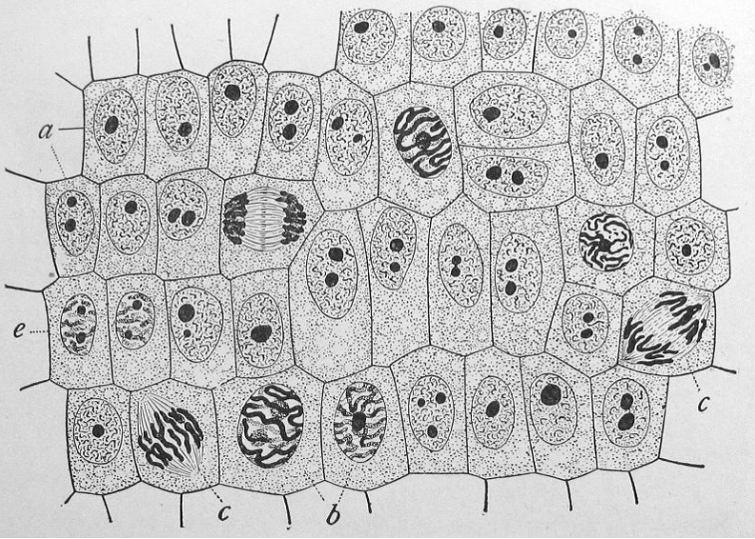
\includegraphics{Images/001.png}
\caption{f.1}
\end{figure}

\textbf{Figure 1.} A 1900 drawing by Edmund Wilson of onion cells at
different stages of mitosis. The sample has been dyed, causing chromatin
in the cells (which soaks up the dye) to appear in greater contrast to
the rest of the cell.

\textbf{图1.} 在1900年Emmund
Wilson在有丝分裂不同阶段绘制的洋葱细胞图。由于样品已被染色,导致细胞中的染色质(吸收染料)与细胞的其他部分形成鲜明对比。

One class of the macromolecules contained in chromatin are called
\textbf{nucleic acids}. Early 20th century research into the chemical
identity of nucleic acids culminated with the conclusion that nucleic
acids are \textbf{polymers}, or repeating chains of smaller, similarly
structured molecules known as \textbf{monomers}. Because of their
tendency to be long and thin, nucleic acid polymers are commonly called
\textbf{strands}.

染色质中含有的一类大分子称为\textbf{核酸}。20世纪早期对核酸化学特性的研究最终得出结论:核酸是\textbf{聚合物},或者将这种重复结构的称为\textbf{单体}。由于它们倾向于长而薄,核酸聚合物通常被称为\textbf{链}。

The nucleic acid monomer is called a \textbf{nucleotide} and is used as
a unit of strand length (abbreviated to nt). Each nucleotide is formed
of three parts: a \textbf{sugar} molecule, a negatively charged
\textbf{ion} called a phosphate, and a compound called a
\textbf{nucleobase} ("base" for short). Polymerization is achieved as
the sugar of one nucleotide bonds to the phosphate of the next
nucleotide in the chain, which forms a \textbf{sugar-phosphate backbone}
for the nucleic acid strand. A key point is that the nucleotides of a
specific type of nucleic acid always contain the same sugar and
phosphate molecules, and they differ only in their choice of base. Thus,
one strand of a nucleic acid can be differentiated from another based
solely on the order of its bases; this ordering of bases defines a
nucleic acid's \textbf{primary structure}.

核酸单体称为\textbf{核苷酸},并作为链长度的单位(缩写为\emph{nt})。每个核苷酸由三部分组成:\textbf{糖分子},带有负离子的\textbf{磷酸盐},和\textbf{核碱基}化合物(简称``碱基'')。当一个核苷酸的糖与链中下一个核苷酸的磷酸键合时开始聚合,其形成核酸链的\textbf{糖-磷酸骨架}。关键点在于特定类型核酸的核苷酸总是含有相同的糖和磷酸盐分子,它们的区别仅在于它们对碱基的选择。因此,核酸的一条链可以仅基于其碱基的顺序与另一条链区分开;碱基的这种排序定义了核酸的\textbf{主要结构}。

For example, Figure 2 shows a strand of \textbf{deoxyribose nucleic
acid} (DNA), in which the sugar is called \textbf{deoxyribose}, and the
only four choices for nucleobases are molecules called \textbf{adenine}
(A), \textbf{cytosine} (C), \textbf{guanine} (G), and \textbf{thymine}
(T).

例如,图2显示了\textbf{脱氧核糖核酸}(DNA)链,其中糖被称为\textbf{脱氧核糖},分别有四种碱基:\textbf{腺嘌呤}(A),\textbf{胞嘧啶}(C),\textbf{鸟嘌呤}(G)和\textbf{胸腺嘧啶}(T)。

\begin{figure}
\centering
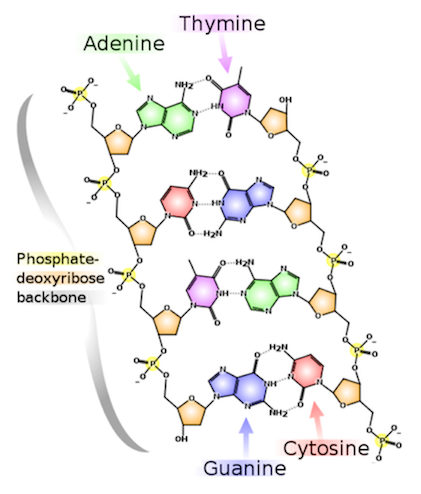
\includegraphics{Images/002.png}
\caption{f.2}
\end{figure}

\textbf{Figure 2.} A sketch of DNA's primary structure.

\textbf{图2.} DNA的主要结构草图。

For reasons we will soon see, DNA is found in all living organisms on
Earth, including bacteria; it is even found in many viruses (which are
often considered to be nonliving). Because of its importance, we reserve
the term \textbf{genome} to refer to the sum total of the DNA contained
in an organism's chromosomes.

DNA存在于地球上的所有生物体中,包括细菌;它甚至存在于许多病毒中(通常被认为是非生命的)。由于其重要性,我们使用``\textbf{基因组}''来指代生物体染色体中包含的DNA的总和。

\subsection{Problem}\label{problem}

\subsection{问题}\label{ux95eeux9898}

A \textbf{string} is simply an ordered collection of symbols selected
from some \textbf{alphabet} and formed into a word; the \textbf{length}
of a string is the number of symbols that it contains.

\textbf{字符串}只是从某些\textbf{字母表}中选择的符号的有序集合,并形成一个单词;字符串的\textbf{长度}是它包含的符号数。

An example of a length 21 \textbf{DNA string} (whose alphabet contains
the symbols 'A', 'C', 'G', and 'T') is "ATGCTTCAGAAAGGTCTTACG."

长度为21的\textbf{DNA串}(其字母包含符号'A','C','G'和'T')的示例是``ATGCTTCAGAAAGGTCTTACG''。

\textbf{Given:} A DNA string s of length at most 1000 nt.

\textbf{Return:} Four integers (separated by spaces) counting the
respective number of times that the symbols 'A', 'C', 'G', and 'T' occur
in s.

\subsection{Sample Dataset}\label{sample-dataset}

\subsection{样本数据集}\label{ux6837ux672cux6570ux636eux96c6}

\begin{verbatim}
AGCTTTTCATTCTGACTGCAACGGGCAATATGTCTCTGTGTGGATTAAAAAAAGAGTGTCTGATAGCAGC
\end{verbatim}

\subsection{Sample Output}\label{sample-output}

\subsection{样本输出}\label{ux6837ux672cux8f93ux51fa}

\begin{verbatim}
20 12 17 21
\end{verbatim}

    \begin{Verbatim}[commandchars=\\\{\}]
{\color{incolor}In [{\color{incolor}3}]:} \PY{k}{def} \PY{n+nf}{count\PYZus{}DNA}\PY{p}{(}\PY{n}{string}\PY{p}{)}\PY{p}{:}
            \PY{n}{c} \PY{o}{=} \PY{p}{\PYZob{}}\PY{l+s+s2}{\PYZdq{}}\PY{l+s+s2}{A}\PY{l+s+s2}{\PYZdq{}}\PY{p}{:}\PY{l+m+mi}{0}\PY{p}{,} \PY{l+s+s2}{\PYZdq{}}\PY{l+s+s2}{C}\PY{l+s+s2}{\PYZdq{}}\PY{p}{:}\PY{l+m+mi}{0}\PY{p}{,} \PY{l+s+s2}{\PYZdq{}}\PY{l+s+s2}{G}\PY{l+s+s2}{\PYZdq{}}\PY{p}{:}\PY{l+m+mi}{0}\PY{p}{,} \PY{l+s+s2}{\PYZdq{}}\PY{l+s+s2}{T}\PY{l+s+s2}{\PYZdq{}}\PY{p}{:}\PY{l+m+mi}{0}\PY{p}{\PYZcb{}}
            \PY{k}{for} \PY{n}{i} \PY{o+ow}{in} \PY{n}{string}\PY{p}{:}
                \PY{k}{if} \PY{n}{i} \PY{o}{==} \PY{l+s+s2}{\PYZdq{}}\PY{l+s+s2}{A}\PY{l+s+s2}{\PYZdq{}}\PY{p}{:}
                    \PY{n}{c}\PY{p}{[}\PY{l+s+s2}{\PYZdq{}}\PY{l+s+s2}{A}\PY{l+s+s2}{\PYZdq{}}\PY{p}{]} \PY{o}{+}\PY{o}{=} \PY{l+m+mi}{1}
                \PY{k}{elif} \PY{n}{i} \PY{o}{==} \PY{l+s+s2}{\PYZdq{}}\PY{l+s+s2}{T}\PY{l+s+s2}{\PYZdq{}}\PY{p}{:}
                    \PY{n}{c}\PY{p}{[}\PY{l+s+s2}{\PYZdq{}}\PY{l+s+s2}{T}\PY{l+s+s2}{\PYZdq{}}\PY{p}{]} \PY{o}{+}\PY{o}{=} \PY{l+m+mi}{1}
                \PY{k}{elif} \PY{n}{i} \PY{o}{==} \PY{l+s+s2}{\PYZdq{}}\PY{l+s+s2}{C}\PY{l+s+s2}{\PYZdq{}}\PY{p}{:}
                    \PY{n}{c}\PY{p}{[}\PY{l+s+s2}{\PYZdq{}}\PY{l+s+s2}{C}\PY{l+s+s2}{\PYZdq{}}\PY{p}{]} \PY{o}{+}\PY{o}{=} \PY{l+m+mi}{1}
                \PY{k}{elif} \PY{n}{i} \PY{o}{==} \PY{l+s+s2}{\PYZdq{}}\PY{l+s+s2}{G}\PY{l+s+s2}{\PYZdq{}}\PY{p}{:}
                    \PY{n}{c}\PY{p}{[}\PY{l+s+s2}{\PYZdq{}}\PY{l+s+s2}{G}\PY{l+s+s2}{\PYZdq{}}\PY{p}{]} \PY{o}{+}\PY{o}{=} \PY{l+m+mi}{1}
            \PY{k}{return} \PY{n}{c}
\end{Verbatim}


    \begin{Verbatim}[commandchars=\\\{\}]
{\color{incolor}In [{\color{incolor}4}]:} \PY{n+nb}{print}\PY{p}{(}\PY{n}{count\PYZus{}DNA}\PY{p}{(}\PY{l+s+s2}{\PYZdq{}}\PY{l+s+s2}{AGCTTTTCATTCTGACTGCAACGGGCAATATGTCTCTGTGTGGATTAAAAAAAGAGTGTCTGATAGCAGC}\PY{l+s+s2}{\PYZdq{}}\PY{p}{)}\PY{p}{)}
\end{Verbatim}


    \begin{Verbatim}[commandchars=\\\{\}]
\{'A': 20, 'C': 12, 'G': 17, 'T': 21\}

    \end{Verbatim}

    \begin{Verbatim}[commandchars=\\\{\}]
{\color{incolor}In [{\color{incolor}5}]:} \PY{k}{with} \PY{n+nb}{open}\PY{p}{(}\PY{l+s+s2}{\PYZdq{}}\PY{l+s+s2}{../Bioinformatics\PYZus{}Stronghold/data/rosalind\PYZus{}dna.txt}\PY{l+s+s2}{\PYZdq{}}\PY{p}{,} \PY{l+s+s2}{\PYZdq{}}\PY{l+s+s2}{r}\PY{l+s+s2}{\PYZdq{}}\PY{p}{)} \PY{k}{as} \PY{n}{r\PYZus{}dna}\PY{p}{:}
            \PY{n}{r\PYZus{}dna} \PY{o}{=} \PY{n}{r\PYZus{}dna}\PY{o}{.}\PY{n}{read}\PY{p}{(}\PY{p}{)}
\end{Verbatim}


    \begin{Verbatim}[commandchars=\\\{\}]
{\color{incolor}In [{\color{incolor}6}]:} \PY{n+nb}{print}\PY{p}{(}\PY{n}{count\PYZus{}DNA}\PY{p}{(}\PY{n}{r\PYZus{}dna}\PY{p}{)}\PY{p}{)}
\end{Verbatim}


    \begin{Verbatim}[commandchars=\\\{\}]
\{'A': 243, 'C': 228, 'G': 221, 'T': 231\}

    \end{Verbatim}

    \begin{Verbatim}[commandchars=\\\{\}]
{\color{incolor}In [{\color{incolor}7}]:} \PY{n}{r\PYZus{}dna}\PY{o}{.}\PY{n}{count}\PY{p}{(}\PY{l+s+s2}{\PYZdq{}}\PY{l+s+s2}{A}\PY{l+s+s2}{\PYZdq{}}\PY{p}{)}
\end{Verbatim}


\begin{Verbatim}[commandchars=\\\{\}]
{\color{outcolor}Out[{\color{outcolor}7}]:} 243
\end{Verbatim}
            
    \section{Transcribing DNA into RNA}\label{transcribing-dna-into-rna}

\section{DNA 转录为 RNA}\label{dna-ux8f6cux5f55ux4e3a-rna}

\subsection{The Second Nucleic Acid}\label{the-second-nucleic-acid}

\subsection{第二种核酸}\label{ux7b2cux4e8cux79cdux6838ux9178}

In ``\textbf{Counting DNA Nucleotides}'', we described the
\textbf{primary structure} of a \textbf{nucleic acid} as a polymer of
\textbf{nucleotide} units, and we mentioned that the omnipresent nucleic
acid \textbf{DNA} is composed of a varied sequence of four bases.

在``\textbf{计数DNA核苷酸}''中,我们描述了\textbf{核酸}的\textbf{一级结构}作为\textbf{核苷酸}单位的聚合物,我们提到了无处不在的核酸\textbf{DNA}由四个碱基的不同序列组成。

Yet a second nucleic acid exists alongside DNA in the
\textbf{chromatin}; this molecule, which possesses a different sugar
called \textbf{ribose}, came to be known as \textbf{ribose nucleic
acid}, or RNA. RNA differs further from DNA in that it contains a base
called \textbf{uracil} in place of \textbf{thymine}; structural
differences between DNA and RNA are shown in Figure 1. Biologists
initially believed that RNA was only contained in plant \textbf{cells},
whereas DNA was restricted to animal cells. However, this hypothesis
dissipated as improved chemical methods discovered both nucleic acids in
the cells of all life forms on Earth.

然而,第二种核酸与\textbf{染色质}中的DNA一起存在;这种分子具有不同的糖,称为\textbf{核糖},后来被称为\textbf{核糖核酸}或RNA。RNA与DNA的不同之处在于它含有一种叫做尿嘧啶的\textbf{碱基代替}胸腺嘧啶\textbf{;DNA和RNA之间的结构差异如图1所示。生物学家最初认为RNA仅包含在}植物细胞**中,而DNA仅限于动物细胞。然而,随着改进的化学方法在地球上所有生命形式的细胞中发现了两种核酸,这一假设消失了。

\begin{figure}
\centering
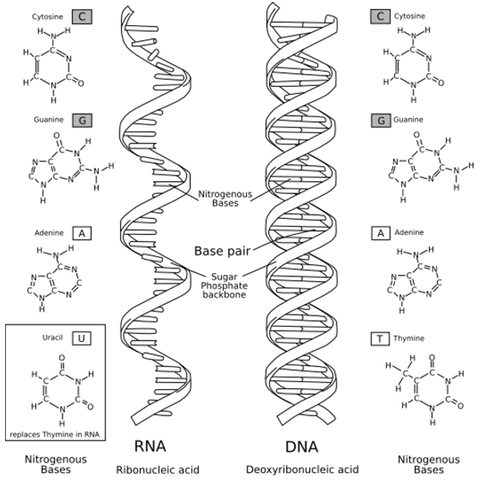
\includegraphics{Images/003.png}
\caption{f.3}
\end{figure}

\textbf{Figure 1.} Structural differences between RNA and DNA

\textbf{图1. } RNA和DNA之间的结构差异

The \textbf{primary structure} of DNA and RNA is so similar because the
former serves as a blueprint for the creation of a special kind of RNA
molecule called \textbf{messenger RNA}, or mRNA. mRNA is created during
RNA transcription, during which a \textbf{strand} of DNA is used as a
template for constructing a strand of RNA by copying nucleotides one at
a time, where uracil is used in place of thymine.

DNA和RNA的\textbf{主要结构}是如此相似,因为前者是创建\textbf{信使RNA}或mRNA这种特殊RNA分子的蓝图。mRNA在RNA转录期间产生,在此期间,DNA的\textbf{链}用作构建RNA链的模板,通过一次复制一个核苷酸,其中使用尿嘧啶代替胸腺嘧啶。

In eukaryotes, DNA remains in the \textbf{nucleus}, while RNA can enter
the far reaches of the cell to carry out DNA's instructions. In future
problems, we will examine the process and ramifications of RNA
transcription in more detail.

在真核生物中,DNA存在于\textbf{细胞核}中,而RNA可以进入细胞的远端以执行DNA的命令。在以后的问题中,我们将更详细地研究RNA转录的过程和分枝。

\subsection{Problem}\label{problem}

An \textbf{RNA string} is a string formed from the alphabet containing
'A', 'C', 'G', and 'U'.

\textbf{RNA串}是由包含'A','C','G'和'U'的字母组成的字符串。

Given a DNA string t corresponding to a coding strand, its transcribed
RNA string u is formed by replacing all occurrences of 'T' in t with 'U'
in u.

给定对应于编码链的DNA串\emph{t},其转录的RNA串\emph{u}通过用\emph{u}中的'U'替换t中所有出现的'T'而形成。

\textbf{Given:} A DNA string t having length at most 1000 nt.

\textbf{Return:} The transcribed RNA string of t.

\subsection{Sample Dataset}\label{sample-dataset}

\begin{verbatim}
GATGGAACTTGACTACGTAAATT
\end{verbatim}

\subsection{Sample Output}\label{sample-output}

\begin{verbatim}
GAUGGAACUUGACUACGUAAAUU
\end{verbatim}

    \begin{Verbatim}[commandchars=\\\{\}]
{\color{incolor}In [{\color{incolor}20}]:} \PY{k}{def} \PY{n+nf}{transcribing\PYZus{}RNA}\PY{p}{(}\PY{n}{string}\PY{p}{)}\PY{p}{:}
             \PY{k}{return} \PY{n}{string}\PY{o}{.}\PY{n}{replace}\PY{p}{(}\PY{l+s+s2}{\PYZdq{}}\PY{l+s+s2}{T}\PY{l+s+s2}{\PYZdq{}}\PY{p}{,} \PY{l+s+s2}{\PYZdq{}}\PY{l+s+s2}{U}\PY{l+s+s2}{\PYZdq{}}\PY{p}{)}
\end{Verbatim}


    \begin{Verbatim}[commandchars=\\\{\}]
{\color{incolor}In [{\color{incolor}21}]:} \PY{n+nb}{print}\PY{p}{(}\PY{n}{transcribing\PYZus{}RNA}\PY{p}{(}\PY{l+s+s2}{\PYZdq{}}\PY{l+s+s2}{GATGGAACTTGACTACGTAAATT}\PY{l+s+s2}{\PYZdq{}}\PY{p}{)}\PY{p}{)}
\end{Verbatim}


    \begin{Verbatim}[commandchars=\\\{\}]
GAUGGAACUUGACUACGUAAAUU

    \end{Verbatim}

    \begin{Verbatim}[commandchars=\\\{\}]
{\color{incolor}In [{\color{incolor}22}]:} \PY{k}{with} \PY{n+nb}{open}\PY{p}{(}\PY{l+s+s2}{\PYZdq{}}\PY{l+s+s2}{../Bioinfo/Bioinformatics\PYZus{}Stronghold/data/rosalind\PYZus{}rna.txt}\PY{l+s+s2}{\PYZdq{}}\PY{p}{)} \PY{k}{as} \PY{n}{rna}\PY{p}{:}
             \PY{n}{rna} \PY{o}{=} \PY{n}{rna}\PY{o}{.}\PY{n}{read}\PY{p}{(}\PY{p}{)}
\end{Verbatim}


    \begin{Verbatim}[commandchars=\\\{\}]
{\color{incolor}In [{\color{incolor}23}]:} \PY{n+nb}{print}\PY{p}{(}\PY{n}{transcribing\PYZus{}RNA}\PY{p}{(}\PY{n}{rna}\PY{p}{)}\PY{p}{)}
\end{Verbatim}


    \begin{Verbatim}[commandchars=\\\{\}]
AACUGCGGCAUCUUAAUCGUGCACUCUUCACAAUGACUACAUGAACAUCAAUUCAGGACGAGGUCUUAUAGCCGGUACUAUGCUUGUCCUGUGAAGGUGCCAUGAGAACAUUGAGAAUAACGCCCCUGGCGCCUUUCACAAUCAUUUCGGGUCACUCCCCAUAUCCGCUAGGGCAACGGUGACGUCUUUCACGAAAUUCAUAGGUAAAGACCGACUUUCAAGCUUGCUAUACGAAUCGCCAGGUCCCUAUUAAACACUAGUAUACAUACACCUCCAGGUGGACCGCGAGUCAAAACAACCAAUUACCUUAGCCUGCAAUCGACCGAGUUAUGGCAGUCCGGAGGAUACGCCGCUCCUCGACCGCAUUUAACUGGUUUGUUGUCACACGAACGCGAUUCUACUGGUAAUUUAAUAUUCUAGAUGCUCUAAGAGCACUUUCUGUGAUGUGAUGCGAAAGGCAUGAACGCUAAACAACUGCCUCGCACAUCACUGUUCACAAGUAGAGCGAUGCCGUGUACUCACAUCAUGCCGUAGUUCUGGUGAUGUUCAGUGCCAGUACAAUGCAUCCUUGGCGCCCGCACGAGCUCCUUGAUAACACUGUGACAGAUAAGGCUAUCUGUAUACCGUCUUCGCGUCCUUCAGGCCUUCAGGGGAAGAGCGCUCAGAGAUACUUGAUCACGAUUCCGCCGGGCUCUGACGGAAUCCAACAGACACAAUUCUAGGCGGUAACCGGCCUUACUUGCGUAUGUGAGUUUCCUGAAAAUGCAUUUUCUAUUGCACCAUGAAUGCCUGGAGAAGUAAUCUCGUCGUCACUCCCAGUCCGACAAGCCAAUAAUCUACCCGCUUUGACUGUGACUAACAACAAUUCUCGCGGGCCGAACGGCAGGACCGGGGUUCGAGACACGAAUCAGCAGGAACAGGCCAGGCCUAGGUAAUGGCUAUGUUCUUGUCG


    \end{Verbatim}


    % Add a bibliography block to the postdoc
    
    
    
    \end{document}
